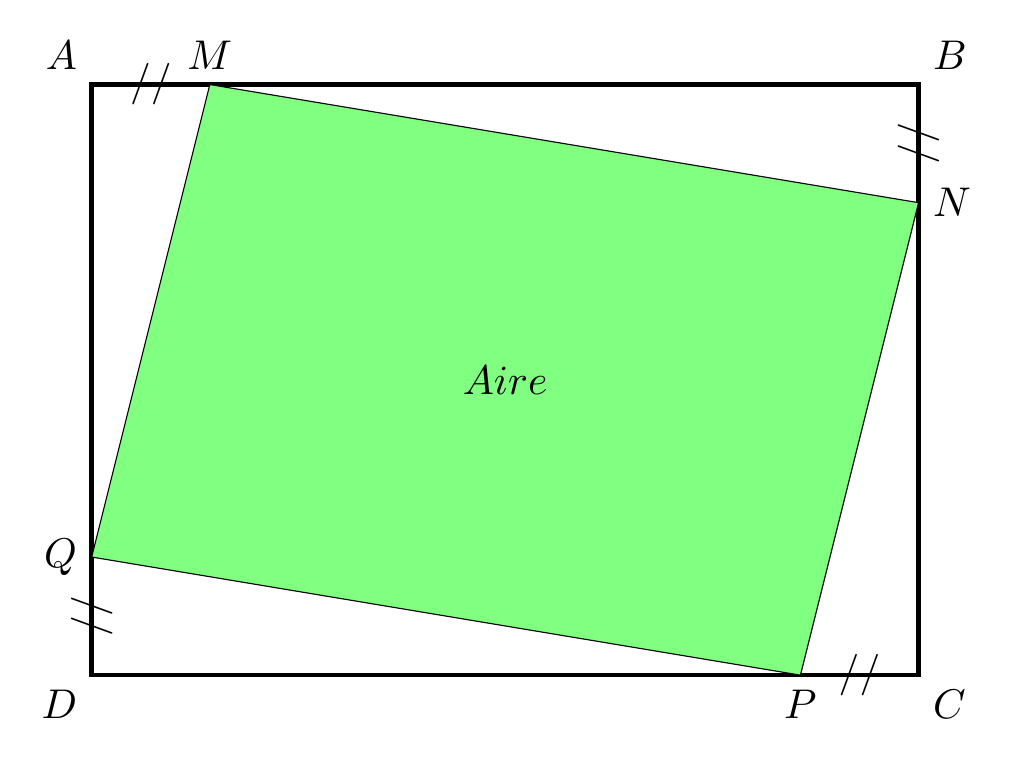
\begin{tikzpicture}[scale=1.5,every node/.style={scale=1.5}]
	\coordinate (A) at (0,0);
	\coordinate (B) at (7,0);
	\coordinate (C) at (7,-5);
	\coordinate (D) at (0,-5);
	\coordinate (M) at (1,0);
	\coordinate (N) at (7,-1);
	\coordinate (P) at (6,-5);
	\coordinate (Q) at (0,-4);
	\coordinate (S) at (7/2,-5/2);
	\draw [ultra thick] (A) rectangle ++(7,-5);
	\draw (A)--(B)--(C)--(D)--cycle;
%	\draw [very thick,red] (A)--(M) node [midway,above] {$x$};
	\draw [black,fill=green!50] (M)--(N)--(P)--(Q)--cycle;
	\draw (A) node[above left] {$A$};
	\draw (B) node[above right] {$B$};
	\draw (C) node[below right] {$C$};
	\draw (D) node[below left] {$D$};
	\draw (M) node[above] {$M$};
	\draw (N) node[right] {$N$};
	\draw (P) node[below] {$P$};
	\draw (Q) node[left] {$Q$};
	\draw (S) node {$Aire$};
%	\foreach \point in {A, B, C, D}
%		\draw (\point) node[above left] {$\point$};
	\draw [black] (A)--(M)node[midway,sloped]{$//$};
	\draw [black] (B)--(N)node[midway,sloped]{$//$};
	\draw [black] (C)--(P)node[midway,sloped]{$//$};
	\draw [black] (D)--(Q)node[midway,sloped]{$//$};
\end{tikzpicture}
